\documentclass[11pt,a4paper]{report}

% ---------- Packages ----------
\usepackage[a4paper,margin=2.5cm]{geometry}
\usepackage[utf8]{inputenc}
\usepackage[T1]{fontenc}
\usepackage{lmodern}
\usepackage{microtype}
\usepackage{xcolor}
\usepackage{booktabs}
\usepackage{longtable}
\usepackage{array}
\usepackage{listings}
\usepackage{amsmath}
\usepackage{amssymb}
\usepackage{graphicx}
\usepackage{hyperref}
\usepackage{enumitem}
\usepackage{tocloft}
\usepackage{fancyhdr}
\usepackage{titlesec}
\usepackage{tikz}
\usetikzlibrary{arrows.meta,positioning,shapes.geometric,fit,backgrounds}
\usepackage[htt]{hyphenat}
\usepackage{seqsplit}

% Allow long, unspaced identifiers (function signatures, dotted paths) inside
% narrow table cells to break instead of overflowing the column.
\setlength{\emergencystretch}{3em}
\tolerance=2000
\hbadness=4000

% ---------- Colors ----------
\definecolor{codebg}{HTML}{0D0D0D}
\definecolor{codefg}{HTML}{E8E8E8}
\definecolor{codecomment}{HTML}{6A9955}
\definecolor{codekeyword}{HTML}{4EC9B0}
\definecolor{codestring}{HTML}{CE9178}
\definecolor{accent}{HTML}{00A8A8}
\definecolor{amber}{HTML}{D96C1E}
\definecolor{tblhead}{HTML}{EAEAEA}

% ---------- Listings setup ----------
\lstdefinelanguage{jsx}{
  morekeywords={const,let,async,await,function,useState,useEffect,export,default,import,from,return,new,if,else,while,for,true,false,null},
  sensitive=true,
  morecomment=[l]{//},
  morecomment=[s]{/*}{*/},
  morestring=[b]',
  morestring=[b]",
  morestring=[b]`
}

\lstset{
  backgroundcolor=\color{codebg},
  basicstyle=\ttfamily\footnotesize\color{codefg},
  keywordstyle=\color{codekeyword}\bfseries,
  commentstyle=\color{codecomment}\itshape,
  stringstyle=\color{codestring},
  numbers=left,
  numberstyle=\tiny\color{gray},
  numbersep=8pt,
  breaklines=true,
  breakatwhitespace=false,
  showstringspaces=false,
  frame=single,
  rulecolor=\color{gray!40},
  framesep=4pt,
  xleftmargin=1.5em,
  tabsize=2,
  captionpos=b,
}

% ---------- Section styling ----------
\titleformat{\chapter}[display]
  {\normalfont\huge\bfseries}{\chaptertitlename\ \thechapter}{20pt}{\Huge\color{black}}
\titleformat{\section}{\normalfont\Large\bfseries\color{black}}{\thesection}{1em}{}
\titleformat{\subsection}{\normalfont\large\bfseries}{\thesubsection}{1em}{}
\titleformat{\subsubsection}{\normalfont\normalsize\bfseries\itshape}{\thesubsubsection}{1em}{}

\hypersetup{
  colorlinks=true,
  linkcolor=accent!70!black,
  citecolor=accent!70!black,
  urlcolor=accent!60!black,
  pdftitle={Mnemos: Technical Documentation},
  pdfauthor={Mnemos Project},
}

\newcolumntype{L}[1]{>{\raggedright\arraybackslash}p{#1}}

\newcommand{\code}[1]{\texttt{\small #1}}
\newcommand{\file}[1]{\texttt{\small\color{accent!70!black}#1}}
\newcommand{\httproute}[2]{\textbf{\texttt{#1}} \texttt{#2}}
% For long, unspaced code (function signatures, dotted paths) inside narrow
% table cells that would otherwise overflow the column — never use in headings.
\newcommand{\bcode}[1]{\texttt{\small\seqsplit{#1}}}

\title{
  {\Huge\bfseries Mnemos}\\[0.3cm]
  {\Large Technical Documentation}\\[0.2cm]
  {\large An Agentic Memory System with Provenance-Tracked Consolidation}
}
\author{Generated Codebase Documentation}
\date{\today}

\begin{document}

\maketitle

\begin{abstract}
\noindent Mnemos is a self-hosted, single-user \emph{agentic memory system} that gives large-language-model assistants persistent, self-consolidating, provenance-tracked memory. It is implemented as a FastAPI backend with a LangGraph-orchestrated ``sleep cycle'' for memory consolidation, an embedded Qdrant vector store paired with a SQLite relational store for full audit trails, a multi-provider LLM abstraction (Groq, Gemini, Ollama), a FastMCP server exposing memory operations as tools to Claude Desktop / Cursor, and a React single-page frontend for chat, memory inspection, roadmap planning, and consolidation-log review. This document provides an exhaustive technical reference to every subsystem: data models, algorithms (decay-ranked retrieval, contradiction resolution, exponential moving-average confidence updates), API contracts, the two LangGraph state machines, the frontend component tree, and the deployment topology.
\end{abstract}

\tableofcontents

% =====================================================================
\chapter{Overview}
% =====================================================================

\section{What Mnemos Is}

Mnemos gives an AI assistant a memory that behaves less like a chat log and more like a human's: raw experiences (\emph{episodes}) are periodically distilled into durable, confidence-weighted \emph{facts}; facts that conflict are adjudicated and superseded rather than silently overwritten; facts that go unused decay in relevance over time; and every fact retains a full chain of provenance back to the episode(s) that produced it.

The system is intentionally \textbf{single-tenant} — there is one implicit user (\code{config: user.default\_user\_id}, default \code{local\_user}) throughout the codebase, with no authentication layer. This is a deliberate simplification appropriate for a personal-assistant deployment (Docker Compose on a single host, or an MCP server running locally beside Claude Desktop).

\section{High-Level Architecture}

\begin{center}
\resizebox{\ifdim\width>\linewidth\linewidth\else\width\fi}{!}{%
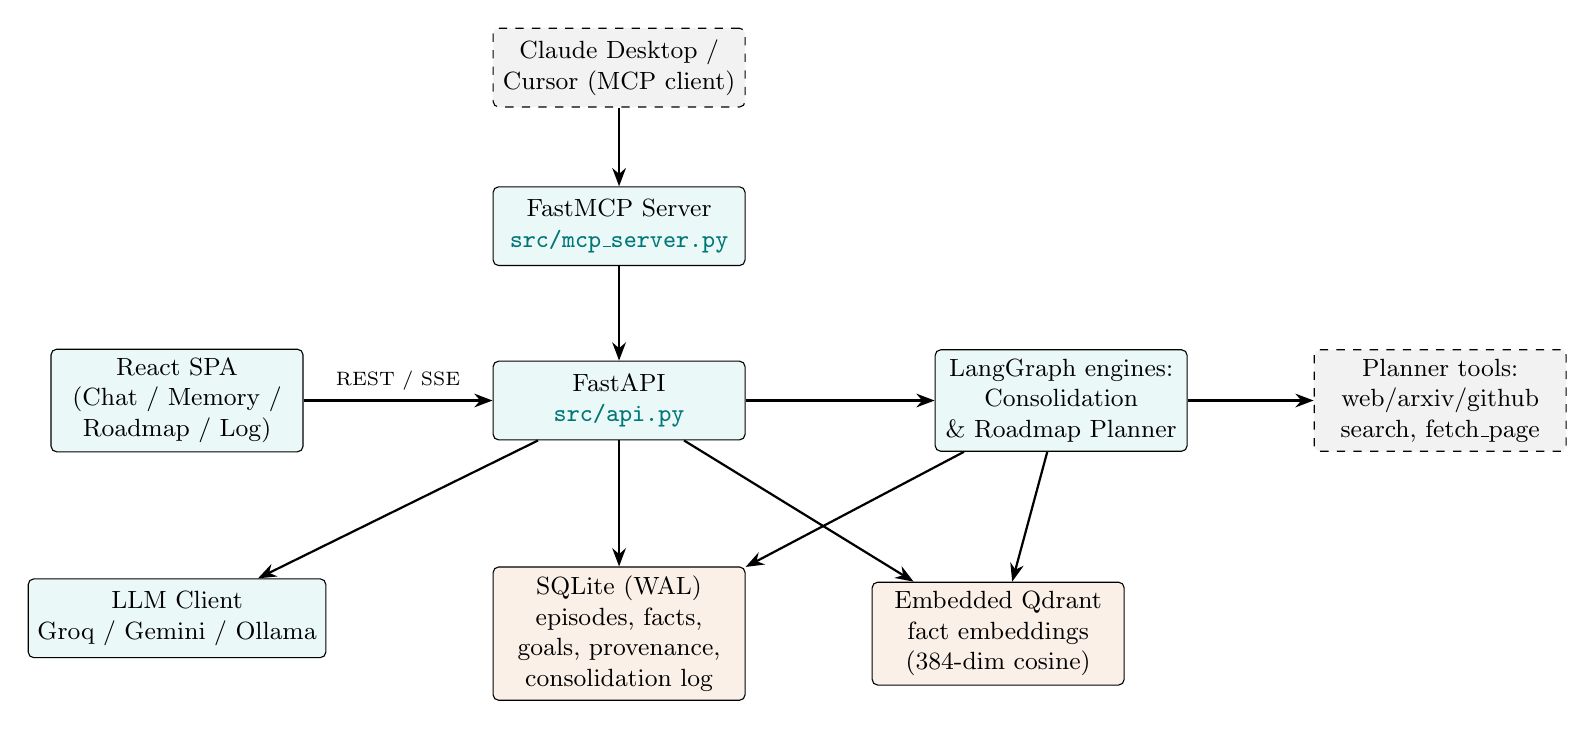
\begin{tikzpicture}[
  box/.style={draw, rounded corners=2pt, minimum width=3.2cm, minimum height=1cm, align=center, font=\small},
  svc/.style={box, fill=accent!8},
  store/.style={box, fill=amber!10},
  ext/.style={box, fill=gray!10, dashed},
  arr/.style={-Stealth, thick}
]
\node[svc] (react) {React SPA\\(Chat / Memory /\\Roadmap / Log)};
\node[svc, right=2.4cm of react] (api) {FastAPI\\\file{src/api.py}};
\node[svc, above=1.2cm of api] (mcp) {FastMCP Server\\\file{src/mcp\_server.py}};
\node[ext, above=1cm of mcp] (claude) {Claude Desktop /\\Cursor (MCP client)};
\node[store, below=1.6cm of api] (sqlite) {SQLite (WAL)\\episodes, facts,\\goals, provenance,\\consolidation log};
\node[store, right=1.6cm of sqlite] (qdrant) {Embedded Qdrant\\fact embeddings\\(384-dim cosine)};
\node[svc, below=1.6cm of react] (llm) {LLM Client\\Groq / Gemini / Ollama};
\node[svc, right=2.4cm of api] (graphs) {LangGraph engines:\\Consolidation \\\& Roadmap Planner};
\node[ext, right=1.6cm of graphs] (tools) {Planner tools:\\web/arxiv/github\\search, fetch\_page};

\draw[arr] (react) -- node[above,font=\scriptsize]{REST / SSE} (api);
\draw[arr] (claude) -- (mcp);
\draw[arr] (mcp) -- (api.north);
\draw[arr] (api) -- (sqlite);
\draw[arr] (api) -- (qdrant);
\draw[arr] (api) -- (llm);
\draw[arr] (api) -- (graphs);
\draw[arr] (graphs) -- (tools);
\draw[arr] (graphs) -- (sqlite);
\draw[arr] (graphs) -- (qdrant);
\end{tikzpicture}%
}
\end{center}

\section{Repository Layout}

\begin{longtable}{L{5.1cm}L{8.6cm}}
\toprule
\textbf{Path} & \textbf{Purpose} \\
\midrule
\endhead
\file{src/api.py} & All FastAPI endpoints (single file, no routers) \\
\file{src/schema.py} & Pydantic v2 domain models \\
\file{src/config.py}, \file{config.yaml} & Configuration loader and tunables \\
\file{src/llm\_client.py} & Multi-provider LLM abstraction \\
\file{src/mcp\_server.py} & FastMCP server (8 tools, 2 resources) \\
\file{src/memory/consolidation.py} & LangGraph ``sleep cycle'' \\
\file{src/memory/contradiction.py} & Contradiction detection \& resolution \\
\file{src/memory/retrieval.py} & Decay-ranked vector retrieval \\
\file{src/planner/roadmap\_planner.py} & Two-node LangGraph roadmap planner \\
\file{src/planner/tools.py} & Research tools bound to the planner LLM \\
\file{src/store/sqlite\_store.py} & Full CRUD over SQLite (WAL mode) \\
\file{src/store/vector\_store.py} & Embedded Qdrant wrapper \\
\file{src/store/embeddings.py} & SentenceTransformer embedding \& cosine similarity \\
\file{frontend/src/App.jsx} & Tab shell: Chat / Memory / Roadmap / Sleep \\
\file{frontend/src/api.js} & All frontend API calls (axios + SSE fetch) \\
\file{frontend/src/panels/*.jsx} & Chat, MemoryInspector, Goals, ConsolidationLog \\
\file{frontend/src/index.css} & Design tokens (HSL variables, zero-radius terminal aesthetic) \\
\file{docker-compose.yml}, \file{Dockerfile}s & Container topology \\
\file{Makefile} & Local dev orchestration \\
\file{pyproject.toml} & Python dependencies (uv/hatchling) \\
\bottomrule
\end{longtable}

% =====================================================================
\chapter{Data Model}
% =====================================================================

All domain models are Pydantic v2 \code{BaseModel} subclasses defined in \file{src/schema.py} (68 lines). Identifiers are all \code{uuid4} strings generated by a shared \code{new\_id()} helper. Two constrained literal types anchor the type system:

\begin{lstlisting}[language=Python,caption={Core literal types (schema.py)}]
FactType = Literal["preference", "status", "event", "skill", "goal", "other"]
GoalStatus = Literal["not_started", "in_progress", "done"]
\end{lstlisting}

\section{Episode}
Raw episodic memory — one turn of interaction or one ingested document.

\begin{longtable}{lll L{6cm}}
\toprule
\textbf{Field} & \textbf{Type} & \textbf{Default} & \textbf{Notes} \\
\midrule
\endhead
\code{episode\_id} & str & \code{uuid4()} & Primary key \\
\code{user\_id} & str & --- & Always the single configured user \\
\code{session\_id} & str & --- & Groups turns of one conversation \\
\code{text} & str & --- & Free text; chat turns stored as \code{"User: ...\textbackslash nAssistant: ..."} \\
\code{timestamp} & datetime & \code{utcnow()} & \\
\bottomrule
\end{longtable}

\section{Fact}
A consolidated, confidence-weighted unit of long-term memory.

\begin{longtable}{lll L{6cm}}
\toprule
\textbf{Field} & \textbf{Type} & \textbf{Default} & \textbf{Notes} \\
\midrule
\endhead
\code{fact\_id} & str & \code{uuid4()} & Primary key \\
\code{content} & str & --- & Full declarative sentence \\
\code{type} & FactType & \code{"other"} & One of the 6 enum values \\
\code{confidence} & float & \code{1.0} & $\in [0,1]$; updated via EMA (\S\ref{sec:ema}) \\
\code{last\_seen} & datetime & \code{utcnow()} & Refreshed on every re-observation \\
\code{metadata} & dict & \code{\{\}} & Free-form \\
\code{superseded\_by} & Optional[str] & \code{None} & Fact ID of the winner, or literal \code{"pruned"} \\
\code{flagged} & bool & \code{False} & Set \code{True} on an unresolved true-tie contradiction \\
\bottomrule
\end{longtable}

\textbf{Facts are never hard-deleted.} Both pruning (confidence below floor) and contradiction resolution mark \code{superseded\_by} rather than removing the row — this is the load-bearing design decision that keeps provenance chains intact indefinitely (\S\ref{sec:provenance-philosophy}).

\section{GoalFact}
One phase of a generated learning roadmap.

\begin{longtable}{lll L{6cm}}
\toprule
\textbf{Field} & \textbf{Type} & \textbf{Default} & \textbf{Notes} \\
\midrule
\endhead
\code{goal\_id} & str & \code{uuid4()} & Primary key \\
\code{user\_id} & str & --- & \\
\code{topic} & str & --- & Roadmap topic, groups phases \\
\code{phase\_index} & int & --- & Ordering within a topic \\
\code{phase\_content} & str & --- & Description of the phase \\
\code{status} & GoalStatus & \code{"not\_started"} & Kanban-style status \\
\code{metadata} & dict & --- & Holds \code{resources: list[str]}, \code{prerequisites: str} \\
\bottomrule
\end{longtable}

\section{Provenance and Log Models}

\begin{itemize}
\item \textbf{\code{FactProvenance}} — junction row \code{(fact\_id, episode\_id)}.
\item \textbf{\code{GoalFactProvenance}} — junction row \code{(goal\_id, episode\_id)}.
\item \textbf{\code{ConsolidationLogEntry}} — audit record of one sleep-cycle run: \code{run\_id}, \code{timestamp}, \code{user\_id}, \bcode{episodes\_processed}, \bcode{facts\_created}, \bcode{facts\_updated}, \bcode{contradictions\_resolved}, \bcode{facts\_pruned}, and \bcode{details: list[dict]} — a free-form event trail (e.g.\ \code{\{"type": "contradiction\_resolved", ...\}} or \code{\{"type": "pruned", ...\}}).
\end{itemize}

\section{Entity-Relationship Diagram}

\begin{center}
\resizebox{\ifdim\width>\linewidth\linewidth\else\width\fi}{!}{%
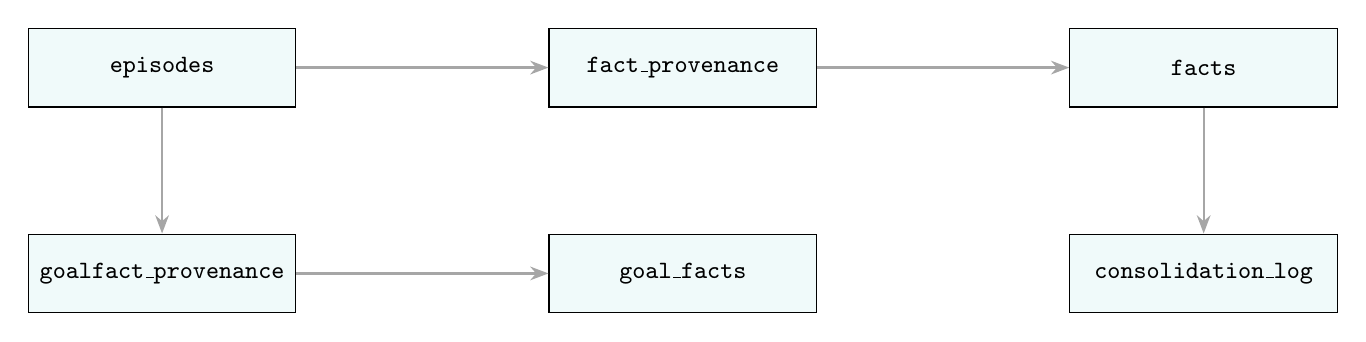
\begin{tikzpicture}[
  ent/.style={draw, minimum width=3.4cm, minimum height=1cm, align=center, font=\small\ttfamily, fill=accent!6},
  rel/.style={-Stealth, thick, color=gray!70}
]
\node[ent] (ep) {episodes};
\node[ent, right=3.2cm of ep] (fp) {fact\_provenance};
\node[ent, right=3.2cm of fp] (fa) {facts};
\node[ent, below=1.6cm of ep] (gp) {goalfact\_provenance};
\node[ent, right=3.2cm of gp] (go) {goal\_facts};
\node[ent, below=1.6cm of fa] (log) {consolidation\_log};

\draw[rel] (ep) -- (fp);
\draw[rel] (fp) -- (fa);
\draw[rel] (ep) -- (gp);
\draw[rel] (gp) -- (go);
\draw[rel] (fa) -- (log);
\end{tikzpicture}%
}
\end{center}

% =====================================================================
\chapter{Storage Layer}
% =====================================================================

Mnemos uses two independent, purpose-fit stores rather than one general database: SQLite for relational/audit data, and an embedded Qdrant instance purely for vector similarity search. There is no ORM — \file{sqlite\_store.py} issues raw SQL via the standard-library \code{sqlite3} module.

\section{SQLite Store (\file{src/store/sqlite\_store.py}, 272 lines)}

Every call opens a connection through a context manager:

\begin{lstlisting}[language=Python,caption={Connection handling}]
@contextmanager
def _conn():
    conn = sqlite3.connect(_DB_PATH)
    conn.row_factory = sqlite3.Row
    conn.execute("PRAGMA journal_mode=WAL")
    conn.execute("PRAGMA foreign_keys=ON")
    try:
        yield conn
        conn.commit()
    except Exception:
        conn.rollback()
        raise
    finally:
        conn.close()
\end{lstlisting}

WAL (write-ahead logging) mode allows concurrent readers alongside a writer, which matters because the FastAPI process and any MCP server process may touch the same database file simultaneously.

\subsection{Schema}

\begin{lstlisting}[language=SQL,caption={Table definitions (init\_db)}]
CREATE TABLE IF NOT EXISTS episodes (
    episode_id TEXT PRIMARY KEY,
    user_id    TEXT,
    session_id TEXT,
    text       TEXT,
    timestamp  TEXT
);

CREATE TABLE IF NOT EXISTS facts (
    fact_id        TEXT PRIMARY KEY,
    content        TEXT,
    type           TEXT DEFAULT 'other',
    confidence     REAL DEFAULT 1.0,
    last_seen      TEXT,
    metadata       TEXT DEFAULT '{}',
    superseded_by  TEXT,
    flagged        INTEGER DEFAULT 0
);

CREATE TABLE IF NOT EXISTS goal_facts (
    goal_id       TEXT PRIMARY KEY,
    user_id       TEXT,
    topic         TEXT,
    phase_index   INTEGER,
    phase_content TEXT,
    status        TEXT DEFAULT 'not_started',
    metadata      TEXT DEFAULT '{}'
);

CREATE TABLE IF NOT EXISTS fact_provenance (
    fact_id    TEXT,
    episode_id TEXT,
    PRIMARY KEY (fact_id, episode_id)
);

CREATE TABLE IF NOT EXISTS goalfact_provenance (
    goal_id    TEXT,
    episode_id TEXT,
    PRIMARY KEY (goal_id, episode_id)
);

CREATE TABLE IF NOT EXISTS consolidation_log (
    run_id               TEXT PRIMARY KEY,
    timestamp            TEXT,
    user_id              TEXT,
    episodes_processed   INTEGER,
    facts_created        INTEGER,
    facts_updated        INTEGER,
    contradictions_resolved INTEGER,
    facts_pruned         INTEGER,
    details              TEXT DEFAULT '[]'
);

CREATE INDEX IF NOT EXISTS idx_episodes_user   ON episodes(user_id);
CREATE INDEX IF NOT EXISTS idx_facts_user_conf ON facts(confidence);
CREATE INDEX IF NOT EXISTS idx_goal_user       ON goal_facts(user_id);
\end{lstlisting}

\begin{quote}\small\itshape
Note: \code{idx\_facts\_user\_conf} is named as though it indexes \code{user\_id}, but it actually indexes \code{confidence} — a naming/implementation mismatch worth fixing if \code{facts} ever needs per-user filtering at scale (currently moot under the single-tenant model).
\end{quote}

\subsection{CRUD Surface}

All writes use \code{INSERT OR REPLACE}, giving upsert semantics keyed on the primary key. Row$\to$model conversion happens through private \code{\_row\_to\_*} helpers that JSON-decode the \code{metadata}/\code{details} columns and ISO-parse timestamps.

\begin{longtable}{L{5.5cm}L{8cm}}
\toprule
\textbf{Function} & \textbf{Behavior} \\
\midrule
\endhead
\code{save\_episode(episode)} & Upsert one episode row \\
\code{get\_episodes(user\_id, limit)} & Most recent $N$ episodes \\
\code{get\_episodes\_since(user\_id, since)} & Episodes newer than a timestamp (drives incremental consolidation) \\
\code{save\_fact(fact)} & Upsert one fact row \\
\code{get\_facts(include\_superseded)} & All facts, optionally filtering out superseded/pruned ones \\
\code{get\_fact(fact\_id)} & Single fact lookup \\
\code{save\_goal\_fact(goal)} / \code{get\_goal\_facts(user\_id)} & Ordered by \code{(topic, phase\_index)} \\
\code{save\_fact\_provenance} & \code{INSERT OR IGNORE} — idempotent link \\
\code{get\_fact\_provenance(fact\_id)} & Returns \code{list[str]} of episode IDs \\
\code{save\_goalfact\_provenance} & Same idempotent pattern for goals \\
\code{save\_consolidation\_log} / \code{get\_consolidation\_log(user\_id, limit=20)} & Audit history \\
\bottomrule
\end{longtable}

\section{Vector Store (\file{src/store/vector\_store.py}, 76 lines)}

Wraps an \textbf{embedded} Qdrant client (\code{QdrantClient(path=...)}, on-disk, no server process) lazily created and memoized in a module global. The collection is created on first use with \code{VectorParams(size=384, distance=Distance.COSINE)}.

Qdrant point IDs must be integers or UUIDs; since fact IDs are UUID \emph{strings}, they are deterministically folded into a 63-bit unsigned integer:

\begin{lstlisting}[language=Python,caption={UUID-to-point-ID conversion}]
def _id_to_uint(uuid_str: str) -> int:
    return uuid.UUID(uuid_str).int % (2 ** 63)
\end{lstlisting}

\begin{longtable}{L{5.5cm}L{8cm}}
\toprule
\textbf{Function} & \textbf{Behavior} \\
\midrule
\endhead
\code{upsert\_fact(fact\_id, embedding, payload)} & Stores the vector with payload merged with \code{\{"fact\_id": fact\_id\}} \\
\bcode{search\_similar(query\_embedding, top\_k=10, score\_threshold=0.0)} & Returns \code{[\{fact\_id, score, payload\}, ...]} via \code{client.query\_points()} \\
\code{delete\_fact(fact\_id)} & Removes the point by its converted ID \\
\bottomrule
\end{longtable}

\section{Embeddings (\file{src/store/embeddings.py}, 33 lines)}

Model: \textbf{\code{sentence-transformers/all-MiniLM-L6-v2}} — 384-dimensional, CPU-only, lazily instantiated once via \code{@lru\_cache(maxsize=1)}.

\begin{lstlisting}[language=Python,caption={Embedding and similarity}]
def embed(text: str) -> list[float]:
    return _model().encode(text, normalize_embeddings=True).tolist()

def embed_batch(texts: list[str]) -> list[list[float]]:
    return _model().encode(texts, batch_size=32,
                            normalize_embeddings=True).tolist()

def cosine_similarity(a, b) -> float:
    return float(np.dot(a, b))   # valid because both vectors are L2-normalized
\end{lstlisting}

Because embeddings are pre-normalized, cosine similarity degenerates to a plain dot product — this is why \code{cosine\_similarity} appears throughout the codebase as a single \code{np.dot} call.

% =====================================================================
\chapter{Memory Subsystem}
% =====================================================================

This is the conceptual core of Mnemos: turning a stream of episodes into a durable, decaying, contradiction-resolved fact base. Three modules cooperate — retrieval, contradiction, and consolidation.

\section{Decay-Ranked Retrieval (\file{src/memory/retrieval.py}, 59 lines)}
\label{sec:retrieval}

Retrieval combines vector similarity with a recency-decay penalty so that older, unused facts naturally fade from context even if they remain semantically relevant.

\subsection{Formula}

Let $q$ be the query embedding, $f$ a candidate fact with embedding $v_f$ and \code{last\_seen} timestamp $t_f$. Let $\Delta t_f$ be the age of the fact in days at query time. The half-life $H$ (default 30 days, \code{memory.decay\_half\_life\_days}) defines a decay constant:
$$
\lambda = \frac{\ln 2}{H}
$$
and the final ranking score is
$$
\text{score}(f) = \underbrace{\cos(q, v_f)}_{\text{semantic similarity}} \times \underbrace{e^{-\lambda \, \Delta t_f}}_{\text{exponential recency decay}}
$$
This halves a fact's effective relevance every $H$ days regardless of how similar it remains to new queries — modeling forgetting as compounding decay rather than a hard cutoff.

\subsection{Implementation}

\begin{lstlisting}[language=Python,caption={retrieve() — over-fetch then decay-rerank}]
_HALF_LIFE_DAYS = get("memory.decay_half_life_days", 30)
_LAMBDA = math.log(2) / _HALF_LIFE_DAYS

def retrieve(query, top_k=5, include_superseded=False):
    query_vec = embeddings.embed(query)
    candidates = vector_store.search_similar(query_vec, top_k=top_k * 3)
    results = []
    for c in candidates:
        fact = sqlite_store.get_fact(c["fact_id"])
        if fact is None or (not include_superseded and fact.superseded_by):
            continue
        age = _age_days(fact)                      # now - last_seen, in days
        score = c["score"] * math.exp(-_LAMBDA * age)
        results.append((fact, score))
    results.sort(key=lambda x: x[1], reverse=True)
    return results[:top_k]
\end{lstlisting}

Two implementation details matter:
\begin{enumerate}
\item Qdrant is asked for $3\times$ the requested \code{top\_k} candidates, because Qdrant itself only ranks by raw cosine similarity — the decay re-ranking happens afterward in Python, and over-fetching guards against a fact that is highly similar but old being pushed out of the candidate pool before decay can be applied.
\item Any exception from the vector store (e.g.\ the collection not existing yet, before the first consolidation run) is caught and yields an empty result rather than propagating — chat still functions with no memory context on a cold start.
\end{enumerate}

\code{retrieve\_for\_context(query, top\_k)} is a thin wrapper returning just \code{list[Fact]} (dropping scores) for direct injection into the chat system prompt.

\section{Contradiction Detection \& Resolution (\file{src/memory/contradiction.py}, 108 lines)}
\label{sec:contradiction}

\subsection{Two-Stage Detection}

A cheap embedding-similarity filter gates an expensive LLM judgment call, so the LLM is only invoked for genuinely plausible conflicts:

\begin{lstlisting}[language=Python,caption={find\_contradictions()}]
def find_contradictions(new_fact: Fact, existing_facts: list[Fact]) -> list[Fact]:
    new_vec = embeddings.embed(new_fact.content)
    conflicts = []
    for ef in existing_facts:
        if ef.fact_id == new_fact.fact_id:
            continue
        ef_vec = embeddings.embed(ef.content)
        sim = embeddings.cosine_similarity(new_vec, ef_vec)
        if sim >= _SIM_THRESHOLD:            # config: memory.similarity_threshold (0.60)
            if _judge_contradiction(new_fact.content, ef.content):
                conflicts.append(ef)
    return conflicts
\end{lstlisting}

The similarity threshold is configured at \code{memory.similarity\_threshold} (0.60 in \file{config.yaml}); the module also defines a code-level fallback default of 0.85 that is only used if the config key is absent. The LLM judge (\code{\_judge\_contradiction}) is few-shot-prompted to distinguish genuine mutual exclusivity (e.g.\ \emph{``is a junior engineer''} vs.\ \emph{``is a senior engineer''}) from compatible statements that merely sound related (e.g.\ \emph{``is vegan''} vs.\ \emph{``doesn't eat meat''}), and must reply with a bare \code{CONTRADICT} or \code{CONSISTENT} token.

\subsection{Resolution Policy}

Given a confirmed contradiction between a new fact and an existing one, resolution proceeds by a strict precedence: confidence, then recency, then an explicit tie state.

\begin{lstlisting}[language=Python,caption={resolve() precedence logic}]
def resolve(new_fact, existing):
    if new_fact.confidence > existing.confidence:
        winner, loser = new_fact, existing
    elif existing.confidence > new_fact.confidence:
        winner, loser = existing, new_fact
    else:
        if new_fact.last_seen > existing.last_seen:
            winner, loser = new_fact, existing
        elif existing.last_seen > new_fact.last_seen:
            winner, loser = existing, new_fact
        else:
            # true tie: flag both, keep both, no supersession
            new_fact.flagged = True
            existing.flagged = True
            save(new_fact); save(existing)
            return new_fact, existing

    loser.superseded_by = winner.fact_id     # soft supersession, never deleted
    save(winner); save(loser)
    return winner, loser
\end{lstlisting}

The loser is never hard-deleted — its row persists with \code{superseded\_by} set to the winner's ID, so provenance queries can still trace back through it. A genuine tie (equal confidence \emph{and} equal \code{last\_seen}) sets \code{flagged = True} on both facts and keeps them side by side for a human to resolve later, surfaced in the UI's fact list.

\section{Consolidation — the ``Sleep Cycle'' (\file{src/memory/consolidation.py}, 265 lines)}
\label{sec:consolidation}

Consolidation is a four-node linear LangGraph that turns a batch of episodes into vetted facts.

\subsection{State Schema}

\begin{lstlisting}[language=Python,caption={ConsolidationState}]
class ConsolidationState(TypedDict):
    user_id: str
    episodes: list[Episode]
    extracted: list[dict]
    new_facts: list[Fact]
    new_fact_ep_ids: dict
    log: ConsolidationLogEntry   # carried as a dict during execution
\end{lstlisting}

\subsection{Graph Wiring}

\begin{lstlisting}[language=Python,caption={Linear consolidation graph}]
g = StateGraph(ConsolidationState)
g.add_node("extract", _extract)
g.add_node("dedupe", _dedupe)
g.add_node("contradiction_check", _contradiction_check)
g.add_node("prune", _prune)
g.set_entry_point("extract")
g.add_edge("extract", "dedupe")
g.add_edge("dedupe", "contradiction_check")
g.add_edge("contradiction_check", "prune")
g.add_edge("prune", END)
\end{lstlisting}

There are no conditional edges — every run passes through all four stages. The compiled graph is memoized once at module load (\code{\_graph}), not recompiled per request.

\begin{center}
\resizebox{\ifdim\width>\linewidth\linewidth\else\width\fi}{!}{%
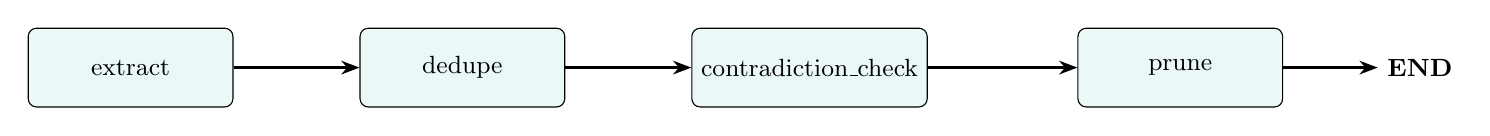
\begin{tikzpicture}[
  node/.style={draw, rounded corners=3pt, minimum width=2.6cm, minimum height=1cm, font=\small, fill=accent!8},
  arr/.style={-Stealth, thick}
]
\node[node] (extract) {extract};
\node[node, right=1.6cm of extract] (dedupe) {dedupe};
\node[node, right=1.6cm of dedupe] (contra) {contradiction\_check};
\node[node, right=1.9cm of contra] (prune) {prune};
\node[draw=none, right=1.2cm of prune, font=\small\bfseries] (end) {END};

\draw[arr] (extract) -- (dedupe);
\draw[arr] (dedupe) -- (contra);
\draw[arr] (contra) -- (prune);
\draw[arr] (prune) -- (end);
\end{tikzpicture}%
}
\end{center}

\subsection{Node 1 — \code{\_extract}}

For each episode, an LLM call is issued with a strict extraction system prompt: emitted facts must be full, standalone sentences (not fragments), each tagged with one of the six \code{FactType} values, and the reply must be a bare JSON array (no prose). The reply is parsed with \code{json.loads}; any per-episode parse failure is silently swallowed (\code{except Exception: pass}) so one malformed LLM response cannot abort the whole batch.

\subsection{Node 2 — \code{\_dedupe}}
\label{sec:ema}

Each extracted candidate fact is embedded and compared by cosine similarity against every existing non-superseded fact; the best match is tracked.

\begin{itemize}
\item If $\text{best\_sim} \ge \text{SIM\_DEDUPE} = 0.92$ (hardcoded — deliberately tighter than the 0.60 contradiction-detection threshold, since deduplication requires near-identical restatement rather than mere topical relatedness), the candidate is treated as a \emph{re-observation} of the matched fact:
$$
\text{confidence}_{\text{new}} = \text{round}\big(w \cdot 1.0 + (1-w)\cdot \text{confidence}_{\text{old}},\ 4\big)
$$
where $w = $ \code{memory.ema\_new\_weight} (default 0.7). This is an exponential moving average that treats each re-observation as a fresh \code{confidence = 1.0} sample, pulling the running confidence toward 1.0 with weight $w$ while retaining $(1-w)$ of the prior value. \code{last\_seen} is refreshed and a new provenance link is added; \code{log.facts\_updated} increments.
\item Otherwise a brand-new \code{Fact} is created (confidence $1.0$, \code{last\_seen} set to the \emph{source episode's own timestamp}, not wall-clock now) and its provenance episode ID is stashed for the next stage; \code{log.facts\_created} increments. New facts are \textbf{not yet persisted} at this point — persistence is deferred to the contradiction-check stage, since a same-run collision between two new facts must still be resolvable.
\end{itemize}

\subsection{Node 3 — \code{\_contradiction\_check}}

For each new candidate fact, \code{contradiction.find\_contradictions()} is run against a \emph{live, continuously updated} view of \code{existing\_facts}:

\begin{itemize}
\item \textbf{Conflict found:} \code{contradiction.resolve()} is invoked; a \code{contradiction\_resolved} detail row is logged (winner/loser IDs and content); the new episode's provenance link is attached to the \emph{winner}; if the winner is the brand-new fact (not previously indexed), it is embedded and upserted into Qdrant now.
\item \textbf{No conflict:} the new fact is persisted directly to SQLite, its provenance saved, its embedding upserted into Qdrant, and it is appended to the local \code{existing\_facts} list.
\end{itemize}

Updating \code{existing\_facts} in place after every resolution is deliberate: it allows two \emph{new} facts extracted within the same consolidation run to contradict each other, not just a new fact against pre-existing memory.

\subsection{Node 4 — \code{\_prune}}

All active (non-superseded) facts are scanned; any with \code{confidence < memory.confidence\_floor} (default $0.1$) are soft-deleted — \code{superseded\_by} is set to the literal string \code{"pruned"} and the corresponding point is removed from the vector index — and a \code{pruned} detail row is logged. The SQLite row itself is never removed.

\subsection{Entry Point}

\begin{lstlisting}[language=Python,caption={run\_consolidation()}]
def run_consolidation(user_id, episodes) -> ConsolidationLogEntry:
    state = {"user_id": user_id, "episodes": episodes, "extracted": [],
             "new_facts": [], "new_fact_ep_ids": {}, "log": {...}}
    final_state = _graph.invoke(state)
    log_entry = ConsolidationLogEntry(**final_state["log"])
    sqlite_store.save_consolidation_log(log_entry)
    return log_entry
\end{lstlisting}

\section{Why Provenance Never Breaks}
\label{sec:provenance-philosophy}

The unifying design principle across retrieval, contradiction, and pruning is that \textbf{no fact row is ever physically deleted}. Superseding (via contradiction) and pruning (via confidence decay) both operate by setting \code{superseded\_by} and removing only the \emph{vector index entry} — the fact remains queryable in SQLite, and every \code{fact\_provenance} link that pointed at it remains valid. This means \code{get\_provenance(fact\_id)} and the MCP \code{get\_provenance} tool can always answer ``why does the assistant believe this / why did it stop believing this'' for the full history of the memory store, not just its current live state.

% =====================================================================
\chapter{LLM Client Abstraction}
% =====================================================================

\section{Uniform Interface (\file{src/llm\_client.py}, 160 lines)}

Every call site in the codebase (chat, extraction, contradiction judging, roadmap synthesis) talks to one of two functions:

\begin{lstlisting}[language=Python,caption={Public interface}]
def chat(messages: list[dict], system: str | None = None,
         temperature: float = 0.2) -> str: ...

def stream(messages: list[dict], system: str | None = None,
           temperature: float = 0.2) -> Iterator[str]: ...
\end{lstlisting}

The active provider is read fresh on every call from \code{config.get("llm.provider", "groq")} and dispatches to a provider-specific implementation. An unrecognized provider name raises \code{ValueError}.

\section{Provider Implementations}

\begin{longtable}{L{2.2cm}L{10.8cm}}
\toprule
\textbf{Provider} & \textbf{Implementation notes} \\
\midrule
\endhead
\textbf{Groq} & \code{groq.Groq} SDK client; model from \code{llm.groq\_model} (default \code{llama-3.1-8b-instant}). Streaming iterates response chunks, pulling \code{chunk.choices[0].delta.content}. \\
\textbf{Gemini} & \code{google.generativeai}; builds \code{GenerativeModel(model\_name, system\_instruction=system)}, converts chat history into \code{\{"role": "user"|"model", "parts":[...]\}} turns, uses \code{start\_chat(history=...)} then \code{send\_message()}. Streaming uses \code{generate\_content(contents, stream=True)}. \\
\textbf{Ollama} & Raw \code{httpx.post} to \code{\{ollama\_base\_url\}/api/chat} (default \code{http://localhost:11434}) with \code{stream: false}/\code{true}; parses \code{.json()["message"]["content"]}, or NDJSON lines when streaming. Requires no API key — fully local. \\
\bottomrule
\end{longtable}

All three SDKs are imported \emph{lazily inside the function body} rather than at module top level, so a deployment using only Groq, for instance, never needs the Gemini or Ollama client libraries installed.

% =====================================================================
\chapter{HTTP API (\file{src/api.py})}
% =====================================================================

FastAPI application, title \emph{``mnemos API v0.1.0''}. On startup (\code{lifespan}), \code{sqlite\_store.init\_db()} runs, and if \code{seed\_demo: true} in \file{config.yaml}, \code{\_seed\_demo()} populates five canned episodes about learning Python and immediately runs consolidation, giving a populated first-run demo. CORS is opened for \code{localhost:5173} (Vite dev) and \code{localhost:3000} (Docker frontend).

\section{Request/Response Models}

Defined inline in \file{api.py} (not in \file{schema.py}):

\begin{lstlisting}[language=Python]
class ChatRequest(BaseModel):
    message: str
    session_id: Optional[str] = None

class ChatResponse(BaseModel):
    reply: str
    session_id: str
    episode_id: str
    memory_used: list[str]

class ConsolidateRequest(BaseModel):
    since_hours: Optional[int] = None

class PlanRequest(BaseModel):
    topic: str
    background: str
    session_id: Optional[str] = None

class IngestRequest(BaseModel):
    source: str
    kind: str = "file"
    session_id: Optional[str] = None
\end{lstlisting}

\section{Endpoint Reference}

\begin{longtable}{L{1.5cm}L{3.2cm}L{8.4cm}}
\toprule
\textbf{Method} & \textbf{Path} & \textbf{Description} \\
\midrule
\endhead
GET & \code{/health} & Liveness probe, returns \code{\{"status": "ok"\}}. \\
POST & \code{/chat} & Retrieves the top-5 decay-ranked facts via \code{retrieval.retrieve\_for\_context}, reconstructs the last 10 episodes of session history, calls \code{llm\_client.chat()} with a system prompt injecting the retrieved memory context, persists the turn as a new \code{Episode}, and invokes \code{\_maybe\_auto\_consolidate()}. \\
POST & \code{/chat/stream} & Same retrieval/history construction as \code{/chat}, but streams tokens over Server-Sent Events as \code{data: \{"token": ...\}}, followed by a final \code{data: \{"done": true, episode\_id, session\_id, memory\_used\}}. Auto-consolidation, if triggered, runs in a background \code{threading.Thread} \emph{after} the done event so it never holds the SSE connection open. \\
GET & \code{/memory/facts} & Query param \code{include\_superseded: bool = False}. Lists facts. \\
GET & \bcode{/memory/fact/\{fact\_id\}} & Returns the fact plus its full list of source episodes (all episodes are loaded once and joined in-memory to avoid N+1 queries). \\
POST & \bcode{/memory/consolidate} & Runs the sleep cycle over episodes since \code{since\_hours}, or the last 500 unconsolidated episodes if omitted. Returns the resulting \code{ConsolidationLogEntry}. \\
GET & \code{/memory/log} & Consolidation run history. \\
POST & \code{/memory/ingest} & Reads a local file (plain text, or PDF via \code{pypdf}, truncated to 8000 characters) or fetches a GitHub repository's metadata + README via the GitHub API, and stores the content as an unconsolidated \code{Episode}. \\
GET & \code{/episodes} & Query param \code{limit: int = 50}. Raw episodic memory listing. \\
GET & \code{/goals} & Lists all \code{GoalFact} roadmap phases. \\
PATCH & \code{/goals/\{goal\_id\}/status} & Query param \code{status: str}; validates membership in \code{\{not\_started, in\_progress, done\}}, returning 404/400 on an unknown ID or invalid status. \\
POST & \code{/plan} & Stores the planning request as an \code{Episode}, invokes \code{plan\_roadmap()} (the researcher+synthesizer LangGraph), and returns the generated phases as \code{GoalFact}s. \\
\bottomrule
\end{longtable}

\section{Auto-Consolidation Trigger}

\begin{lstlisting}[language=Python,caption={\_maybe\_auto\_consolidate() logic}]
def _maybe_auto_consolidate():
    trigger = get("consolidation.trigger", "manual")   # manual | end_of_session | both
    if trigger == "manual":
        return
    last_run = sqlite_store.get_consolidation_log(_USER_ID, limit=1)
    since = last_run[0].timestamp if last_run else None
    new_episodes = sqlite_store.get_episodes_since(_USER_ID, since) if since \
                   else sqlite_store.get_episodes(_USER_ID, limit=10_000)
    if len(new_episodes) >= get("consolidation.min_episodes_to_trigger", 3):
        run_consolidation(_USER_ID, new_episodes)
\end{lstlisting}

\section{Ingestion Duplication}

Note that file/GitHub ingestion logic is implemented \emph{twice} — once inline within the \code{/memory/ingest} REST endpoint, and once as the independent MCP tools \code{ingest\_file}/\code{ingest\_github} (\S\ref{sec:mcp}). Both use the same 8000-character truncation and the same \code{\_TEXT\_SUFFIXES} allow-list, but are not factored into a shared module — a candidate for future consolidation of the codebase itself.

% =====================================================================
\chapter{MCP Server}
% =====================================================================

\label{sec:mcp}
\section{Purpose and Transport}

\file{src/mcp\_server.py} (417 lines) exposes the same underlying memory operations as first-class tools for MCP-compatible clients (Claude Desktop, Cursor), independent of the REST API. Built with \code{FastMCP(name="mnemos", instructions=...)}. Two transport modes:

\begin{lstlisting}[language=bash,caption={Running the MCP server}]
uv run python -m src.mcp_server                    # stdio (Claude Desktop)
uv run python -m src.mcp_server --http --port 8001  # HTTP/SSE
\end{lstlisting}

\section{Tools}

\begin{longtable}{L{4.8cm}L{7.5cm}}
\toprule
\textbf{Tool} & \textbf{Description} \\
\midrule
\endhead
\bcode{remember(text, session\_id="mcp\_session")} & Stores an \code{Episode}; returns a confirmation string containing the new \code{episode\_id}. \\
\code{recall(query, top\_k=5)} & Calls \code{retrieval.retrieve()}; formats a ranked list including type, confidence, decay-adjusted score, last-seen, and a flagged marker. \\
\code{get\_provenance(fact\_id)} & Traces a fact back to its source episodes; formats timestamps, session IDs, and truncated (300-char) episode text. \\
\code{consolidate()} & Runs the sleep cycle over up to 500 episodes; returns a formatted summary of the resulting \code{ConsolidationLogEntry}. \\
\bcode{list\_facts(include\_flagged=True)} & Lists all non-superseded facts sorted by confidence descending, with an optional flagged-only filter. \\
\bcode{plan\_learning\_roadmap(topic, background)} & Invokes \code{plan\_roadmap()}; formats phases with resources, status, and goal ID. \\
\bcode{ingest\_file(path, session\_id="file\_ingest")} & Reads a local text/PDF file (same 8000-char truncation and suffix allow-list as the REST endpoint) and stores it as an Episode. \\
\bcode{ingest\_github(repo\_url, session\_id="github\_ingest")} & Regex-parses owner/repo from the URL, fetches GitHub API metadata + README (optional \code{GITHUB\_TOKEN} bearer auth), stores as an Episode. \\
\bottomrule
\end{longtable}

\section{Resources}

\begin{longtable}{L{4.8cm}L{7.5cm}}
\toprule
\textbf{Resource URI} & \textbf{Content} \\
\midrule
\endhead
\code{memory://facts} & Markdown table of all active facts: \code{| Type | Confidence | Last Seen | Content |}. \\
\code{memory://consolidation-log} & Plain-text summary of the 10 most recent consolidation runs, one line per run. \\
\bottomrule
\end{longtable}

% =====================================================================
\chapter{Roadmap Planner}
% =====================================================================

\section{Purpose}

Given a topic and the user's background, \file{src/planner/roadmap\_planner.py} (240 lines) produces a multi-phase learning roadmap grounded in live web/arXiv/GitHub research rather than pure LLM recall, via a two-node LangGraph.

\section{State Schema}

\begin{lstlisting}[language=Python,caption={PlannerState}]
class PlannerState(TypedDict):
    messages: Annotated[list, operator.add]   # LangGraph auto-accumulates
    topic: str
    background: str
    raw_plan: str        # JSON string produced by the synthesizer
\end{lstlisting}

\section{Graph Wiring}

\begin{lstlisting}[language=Python]
g = StateGraph(PlannerState)
g.add_node("researcher", _researcher)
g.add_node("synthesizer", _synthesizer)
g.set_entry_point("researcher")
g.add_edge("researcher", "synthesizer")
g.add_edge("synthesizer", END)
\end{lstlisting}

\begin{center}
\resizebox{\ifdim\width>\linewidth\linewidth\else\width\fi}{!}{%
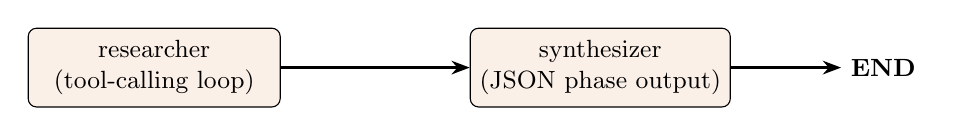
\begin{tikzpicture}[
  node/.style={draw, rounded corners=3pt, minimum width=3.2cm, minimum height=1cm, align=center, font=\small, fill=amber!10},
  arr/.style={-Stealth, thick}
]
\node[node] (res) {researcher\\(tool-calling loop)};
\node[node, right=2.4cm of res] (syn) {synthesizer\\(JSON phase output)};
\node[draw=none, right=1.4cm of syn, font=\small\bfseries] (end) {END};
\draw[arr] (res) -- (syn);
\draw[arr] (syn) -- (end);
\end{tikzpicture}%
}
\end{center}

\section{Node 1 — Researcher}

Builds a tool-bound chat model via \code{\_get\_llm\_with\_tools()} — either \code{ChatGroq} or \code{ChatGoogleGenerativeAI} with \code{.bind\_tools(PLANNER\_TOOLS)}. Ollama is explicitly unsupported here (\code{ValueError}) since the local integration used does not support tool calling. Runs an agentic loop capped at 8 iterations:

\begin{lstlisting}[language=Python,caption={Agentic tool-calling loop (simplified)}]
for _ in range(8):
    response = llm.invoke(messages)
    messages.append(response)
    if not response.tool_calls:
        break
    tool_results = ToolNode(PLANNER_TOOLS).invoke(messages)
    messages.extend(tool_results)
return {"messages": messages[2:]}   # drop initial system/human turns
\end{lstlisting}

The system prompt instructs 5–8 total tool calls: \code{web\_search} for learning resources, \code{github\_search} for reference repositories, \code{arxiv\_search} at least twice with distinct CS category codes, and an optional \code{fetch\_page} for deeper reading. Returning \code{messages[2:]} avoids LangGraph's \code{operator.add} reducer duplicating the initial system/human turns in the accumulated state.

\section{Node 2 — Synthesizer}

Builds a \emph{fresh}, non-tool-bound LLM at \code{temperature=0.0} (deterministic structured output), concatenates all AI/tool message content from the research history (capped to the last 6000 characters), and prompts for a strict JSON array of 4–6 phases:

\begin{lstlisting}[caption={Synthesizer output shape}]
[
  {
    "phase_index": 0,
    "phase_content": "...",
    "resources": ["https://...", "..."],
    "prerequisites": "..."
  }
]
\end{lstlisting}

The prompt explicitly forbids repeating the same resource URL across phases.

\section{Post-Processing (\code{plan\_roadmap})}

\begin{lstlisting}[language=Python,caption={plan\_roadmap() signature}]
def plan_roadmap(topic: str, background: str, user_id: str | None = None,
                  source_episode_id: str | None = None) -> list[GoalFact]:
    ...
\end{lstlisting}

After invoking the graph: markdown code fences are stripped from \code{raw\_plan}; \code{json.loads} is attempted, falling back to a regex \code{\textbackslash[.*\textbackslash]} extraction if parsing fails; a \textbf{cross-phase URL dedup pass} runs in Python, normalizing arXiv URLs by stripping trailing version suffixes (\code{rstrip("v0123456789")}) so \code{.../2301.01234v1} and \code{.../2301.01234v2} are recognized as the same resource; each phase becomes a \code{GoalFact} (\code{status="not\_started"}) persisted via \code{sqlite\_store.save\_goal\_fact}, optionally linked to \code{source\_episode\_id} for provenance.

\section{Research Tools (\file{src/planner/tools.py}, 182 lines)}

LangChain \code{@tool}-decorated functions bound to the researcher LLM as \code{PLANNER\_TOOLS}.

\begin{longtable}{L{3.6cm}L{8.7cm}}
\toprule
\textbf{Tool} & \textbf{Behavior} \\
\midrule
\endhead
\code{web\_search(query)} & Tavily API (\code{TAVILY\_API\_KEY}, max 5 results); silently falls back to \bcode{duckduckgo\_search.DDGS().text()} on any exception or missing key. \\
\code{github\_search(query)} & GitHub REST \bcode{search/repositories?sort=stars\&order=desc\&per\_page=5}, optional \code{GITHUB\_TOKEN} bearer auth; formats name/stars/description/topics/URL. \\
\code{fetch\_page(url)} & \code{httpx.get} with a custom User-Agent; BeautifulSoup strips \bcode{script/style/nav/footer/header}, collapses whitespace, truncates to 3000 characters via \code{textwrap.shorten}. \\
\bcode{arxiv\_search(query, categories="cs.LG cs.AI cs.CL stat.ML")} & Builds a scoped query \code{(query) AND (cat:X OR cat:Y ...)}; uses \code{arxiv.Client()} / \bcode{arxiv.Search(sort\_by=Relevance, max\_results=10)}; post-filters to a hardcoded category allow-list (\bcode{cs.LG, cs.AI, cs.CL, cs.CV, cs.NE, cs.IR, cs.HC, cs.RO, cs.SE, cs.CR, stat.ML, econ.EM, q-bio.NC}); returns up to 4 results (title, categories, authors, published date, cleaned URL, abstract). Falls back to an unfiltered search if category filtering yields zero results. \\
\bottomrule
\end{longtable}

% =====================================================================
\chapter{Configuration}
% =====================================================================

\section{Loader (\file{src/config.py}, 41 lines)}

\begin{lstlisting}[language=Python,caption={Config loading}]
@lru_cache(maxsize=1)
def load_config() -> dict:
    ...  # loads config.yaml once, resolves database/vector_store paths
         # to absolute paths against the repo root

def get(key_path: str, default=None):
    ...  # dotted-path lookup, e.g. get("memory.ema_new_weight")

def api_key(provider: str) -> str | None:
    # groq -> GROQ_API_KEY, gemini -> GOOGLE_API_KEY env vars
    # ollama needs no key
\end{lstlisting}

\code{.env} is loaded via \code{python-dotenv} at import time. Path resolution anchors on \code{\_ROOT = Path(\_\_file\_\_).parent.parent} so relative paths in \file{config.yaml} always resolve consistently regardless of the process's working directory.

\section{Full Tunable Reference}

\begin{lstlisting}[caption={config.yaml}]
llm:
  provider: groq              # groq | gemini | ollama
  groq_model: llama-3.1-8b-instant
  gemini_model: gemini-1.5-flash
  ollama_model: llama3
  ollama_base_url: http://localhost:11434
embeddings:
  model: all-MiniLM-L6-v2      # sentence-transformers, CPU
  dimension: 384
vector_store:
  path: ./data/qdrant
  collection: mnemos_facts
database:
  path: ./data/mnemos.db
memory:
  ema_new_weight: 0.7            # EMA weight toward a fresh observation
  decay_half_life_days: 30       # retrieval recency half-life
  confidence_floor: 0.1          # prune threshold
  similarity_threshold: 0.60     # contradiction pre-filter (cosine)
consolidation:
  trigger: manual                 # manual | end_of_session | both
  min_episodes_to_trigger: 3
user:
  default_user_id: local_user
seed_demo: false
\end{lstlisting}

\begin{quote}\small\itshape
\textbf{Documented inconsistency.} The frontend footer status bar (\file{App.jsx}) displays static, hardcoded pipeline parameters (\emph{t\textonehalf\ 168h}, \emph{sim\,$\geq$\,0.85}, \emph{floor 0.15}) that do not match the values actually in force per \file{config.yaml} (30-day half-life, 0.60 similarity threshold, 0.10 confidence floor). These display values are not live-fetched from \code{/health} or any config endpoint — a UI/documentation gap rather than a functional bug, since the backend always uses the real \file{config.yaml} values regardless of what the footer displays.
\end{quote}

% =====================================================================
\chapter{Frontend}
% =====================================================================

React 19 + Vite, JSX only (no TypeScript), no CSS framework — all styling is hand-written CSS using HSL custom properties.

\section{Application Shell (\file{App.jsx}, 59 lines)}

Four tabs — \code{chat}, \code{memory}, \code{roadmap}, \code{log} — rendered respectively as \code{Chat}, \code{MemoryInspector}, \code{Goals}, \code{ConsolidationLog}. A single \code{SESSION\_ID = crypto.randomUUID()} is generated once at module scope per page load (not per render), scoping all chat activity for that browser tab to one session.

\section{API Layer (\file{api.js}, 65 lines)}

A thin \code{axios} wrapper (\code{baseURL: ''}), relying on the Vite dev-server proxy (or, in Docker, nginx) to forward \code{/chat}, \code{/memory}, \code{/episodes}, \code{/goals}, \code{/plan}, \code{/health} to the backend on the same origin.

\begin{lstlisting}[language=jsx,caption={Hand-rolled SSE stream reader}]
export async function streamMessage(message, sessionId, onToken, onDone) {
  const res = await fetch('/chat/stream', {
    method: 'POST',
    headers: { 'Content-Type': 'application/json' },
    body: JSON.stringify({ message, session_id: sessionId }),
  });
  const reader = res.body.getReader();
  const decoder = new TextDecoder();
  let buffer = '';
  while (true) {
    const { done, value } = await reader.read();
    if (done) break;
    buffer += decoder.decode(value, { stream: true });
    const lines = buffer.split('\n');
    buffer = lines.pop();               // retain partial trailing line
    for (const line of lines) {
      if (!line.startsWith('data: ')) continue;
      const payload = JSON.parse(line.slice(6));
      if (payload.done) onDone(payload);
      else onToken(payload.token);
    }
  }
}
\end{lstlisting}

Other exported functions: \code{sendMessage}, \code{getFacts}, \code{getFactWithProvenance}, \code{triggerConsolidate}, \code{getConsolidationLog}, \code{getEpisodes}, \code{getGoals}, \code{updateGoalStatus}, \code{createRoadmap}, \code{ingestSource}.

\section{Panels}

\subsection{Chat (\file{panels/Chat.jsx}, 301 lines)}
Streaming message list where assistant replies grow token-by-token via the \code{streamMessage} callback appending to the last message's content. Each assistant message has an expandable ``memory'' panel showing the \code{fact\_id}/content/score that informed that specific reply. A collapsible ``ctx'' strip at the top shows the top-8 facts loaded on mount (\code{getFacts()}). Supports copy-to-clipboard per message, an auto-resizing textarea, Enter-to-send, and a roadmap-generation modal (topic + background $\to$ \code{createRoadmap}). \code{confBar(conf)} maps a confidence value to an HSL teal color for the visual confidence bars.

\subsection{Memory Inspector (\file{panels/MemoryInspector.jsx}, 188 lines)}
A toolbar with a file/GitHub ingest form (\code{ingestSource}), type-filter pills (\code{all/preference/skill/status/event/goal/other}), and a manual ``consolidate'' trigger. The main view is a fact table (type, content, confidence \%, age) whose rows expand on click to reveal confidence, last-seen, source count, the raw \code{fact\_id}, and the full list of provenance episodes (lazily fetched via \code{getFactWithProvenance}).

\subsection{Goals (\file{panels/Goals.jsx}, 122 lines)}
A three-column Kanban board — \code{TODO}/\code{ACTIVE}/\code{DONE} mapped to \code{not\_started}/\code{in\_progress}/\code{done} — with cards grouped by topic and ordered by \code{phase\_index} within each status column. Each card shows the topic, phase description, up to two resource links, and status-transition buttons (\code{updateGoalStatus}). The top bar reports topic count and a done/total completion fraction.

\subsection{Consolidation Log (\file{panels/ConsolidationLog.jsx}, 135 lines)}
A timeline of consolidation runs; each entry expands into a synthetic ``terminal log'' view (\code{buildLogLines}) rendering the four pipeline stages (\code{extract $\to$ dedupe $\to$ contradict $\to$ prune}) with their respective counts, plus up to two contradiction-detail lines showing the winning fact's content. Includes a ``run now'' button wired to \code{triggerConsolidate}.

\section{Design System (\file{index.css}, 68 lines)}

Fonts: IBM Plex Sans (UI text) and IBM Plex Mono (data/numeric values). The palette is a dark, zero-radius ``terminal'' aesthetic:

\begin{lstlisting}[caption={Root design tokens}]
:root {
  --bg:  hsl(0,   0%,  2%);   /* page background, near-black       */
  --s1:  hsl(0,   0%,  5%);   /* surface 1                          */
  --s2:  hsl(0,   0%,  8%);   /* surface 2                          */
  --s3:  hsl(0,   0%, 12%);   /* surface 3                          */
  --b1:  hsl(0,   0%, 14%);   /* border 1                           */
  --b2:  hsl(0,   0%, 24%);   /* border 2                           */
  --b3:  hsl(0,   0%, 38%);   /* border 3                           */
  --t1:  hsl(0,   0%, 95%);   /* text primary                       */
  --t2:  hsl(0,   0%, 68%);   /* text secondary                     */
  --t3:  hsl(0,   0%, 46%);   /* text tertiary                      */
  --t4:  hsl(0,   0%, 28%);   /* text quaternary / dim              */
  --ac:  hsl(180, 100%, 50%); /* accent -- teal / cyan              */
  --am:  hsl(24,  100%, 58%); /* amber -- logo underscore, warnings */
  --gr:  hsl(140, 80%,  48%); /* green -- success / ok              */
  --re:  hsl(0,   90%,  60%); /* red -- error                       */
  --f:   'IBM Plex Sans', system-ui, sans-serif;
  --fm:  'IBM Plex Mono', monospace;
  --tx: 11px; --ts: 12px; --tm: 13px; --tl: 14px; --txl: 15px;  /* type scale */
  --r:  0px;  --rl: 0px;      /* border-radius: none, anywhere      */
}
\end{lstlisting}

Confidence visualizations elsewhere reuse the accent hue: \code{hsl(180, saturation=conf\%, lightness=18+conf*32)}, so higher-confidence facts render as more saturated, brighter teal bars.

% =====================================================================
\chapter{Deployment \& Tooling}
% =====================================================================

\section{Docker Compose Topology}

\begin{lstlisting}[caption={docker-compose.yml (structure)}]
services:
  backend:
    build: .
    env_file: .env
    volumes: ["./data:/app/data"]
    ports: ["8000:8000"]
    healthcheck: curl -f http://localhost:8000/health

  frontend:
    build: ./frontend
    ports: ["3000:80"]
    depends_on:
      backend:
        condition: service_healthy
\end{lstlisting}

\section{Backend Dockerfile}

Base image \code{python:3.11-slim}; installs \code{curl} (for the healthcheck) and \code{uv}. Three cache-friendly layers:
\begin{enumerate}
\item \code{uv sync --frozen --no-install-project} run against just \file{pyproject.toml}/\file{uv.lock}, copied first — so dependency installation is cached across code-only changes.
\item The \code{all-MiniLM-L6-v2} embedding model is baked into the image at \emph{build time} (\code{python -c "SentenceTransformer(...)"}), so container cold-starts never pay the model-download cost.
\item \file{src/} and \file{config.yaml} are copied last, since they change most often.
\end{enumerate}
Entrypoint: \code{uvicorn src.api:app --host 0.0.0.0 --port 8000}; healthcheck runs every 15 seconds.

\section{Frontend Dockerfile}

Multi-stage: a \code{node:20-alpine} builder stage runs \code{npm ci} then \code{npm run build} (Vite), followed by an \code{nginx:alpine} runtime stage serving \code{/app/dist} with a custom \code{nginx.conf}; healthcheck via \code{wget}.

\section{Local Development (\file{Makefile})}

\begin{lstlisting}[caption={Makefile targets}]
install:  # uv sync + npm install
dev:      # runs backend and frontend concurrently (bash), trap 'kill 0' EXIT
backend:  # uv run uvicorn src.api:app --reload   -> :8000
frontend: # cd frontend && npm run dev             -> :5173
\end{lstlisting}

\section{Python Dependencies (\file{pyproject.toml})}

Package \code{mnemos 0.1.0}, requires Python $\geq 3.11$, build backend \code{hatchling}.

\begin{longtable}{L{6.5cm}L{6.5cm}}
\toprule
\textbf{Category} & \textbf{Packages} \\
\midrule
\endhead
Web framework & \code{fastapi}, \code{uvicorn[standard]}, \code{pydantic>=2.7} \\
Config/env & \code{python-dotenv}, \code{pyyaml} \\
LLM providers & \code{groq}, \code{google-generativeai} \\
Embeddings/vectors & \code{sentence-transformers}, \code{qdrant-client}, \code{numpy} \\
Orchestration & \code{langgraph}, \code{langchain-core}, \code{langchain-groq}, \code{langchain-google-genai}, \code{langgraph-prebuilt} \\
Research tools & \code{httpx}, \code{duckduckgo-search}, \code{arxiv}, \code{beautifulsoup4} \\
MCP \& docs & \code{fastmcp}, \code{pypdf} \\
Dev tooling & \code{pytest}, \code{pytest-asyncio}, \code{ruff} (dev extras) \\
\bottomrule
\end{longtable}

Console script: \code{mnemos-mcp = src.mcp\_server:mcp.run}. Ruff is configured with \code{line-length = 100}, \code{target-version = "py311"}.

\section{Environment Variables}

\begin{longtable}{L{3.5cm}L{2cm}L{6.5cm}}
\toprule
\textbf{Variable} & \textbf{Required} & \textbf{Notes} \\
\midrule
\endhead
\code{GROQ\_API\_KEY} & At least one LLM key & Free tier available \\
\code{GOOGLE\_API\_KEY} & At least one LLM key & Gemini free tier \\
\code{TAVILY\_API\_KEY} & Optional & Web search; DuckDuckGo fallback if absent \\
\code{GITHUB\_TOKEN} & Optional & Raises GitHub API rate limit from 60 to 5000 req/hr \\
\code{LANGSMITH\_API\_KEY} & Optional & LangSmith tracing \\
\code{LANGCHAIN\_TRACING\_V2} & Optional & Enables LangSmith tracing \\
\code{LANGCHAIN\_PROJECT} & Optional & LangSmith project name \\
\bottomrule
\end{longtable}

Ollama requires no API key since it runs entirely locally.

% =====================================================================
\chapter{Cross-Cutting Observations}
% =====================================================================

\begin{enumerate}
\item \textbf{Single-tenant by design.} \code{user\_id} is always the same config-driven constant throughout \file{api.py} and \file{mcp\_server.py}; there is no authentication or multi-tenancy layer anywhere in the system. This is appropriate for a personal, self-hosted deployment but would need to be introduced before any multi-user use case.
\item \textbf{Duplicated ingestion logic.} File and GitHub ingestion are implemented independently in the REST \code{/memory/ingest} endpoint and in the MCP \code{ingest\_file}/\code{ingest\_github} tools, sharing constants (the 8000-char truncation limit, the text-suffix allow-list) but not a common code path.
\item \textbf{Provenance is permanent.} Both pruning and contradiction resolution use soft-supersession (\code{superseded\_by}) rather than deletion — see \S\ref{sec:provenance-philosophy}. This is the central architectural commitment of the memory subsystem.
\item \textbf{Both LangGraph graphs are compiled once.} The consolidation graph (\S\ref{sec:consolidation}) and the roadmap planner graph (Chapter~7) are each memoized at module load into a module-level global, not recompiled per request.
\item \textbf{Config/UI drift.} The frontend footer's displayed pipeline parameters do not match \file{config.yaml}'s actual values (\S6.2) — a cosmetic inconsistency, not a functional one, since the backend always reads the real config.
\item \textbf{Threshold asymmetry is intentional.} The 0.92 hardcoded deduplication threshold in \code{\_dedupe} is deliberately tighter than the 0.60 configured contradiction-detection threshold: deduplication requires near-verbatim restatement, while contradiction detection needs only topical relatedness before the LLM judge is asked to confirm genuine conflict.
\end{enumerate}

\end{document}
